\documentclass[12pt]{article}
\usepackage{setspace}
\setlength{\parindent}{4em}
\usepackage{fancyvrb}
\usepackage{graphicx}
\usepackage{geometry}
\renewcommand\thesection{\arabic{section}}
\renewcommand\thesubsection{\thesection.\arabic{subsection}}
\geometry{letterpaper, portrait, margin=1in}

%%%Title Page%%%
\title{\vspace{3cm}Lab 02\bigbreak 4-bit ALU}
\author{
{\normalsize
\begin{tabular}{l r r}
 & \textbf{Ryan Cruz} & \textbf{Zachary Davis}\\
\textbf{Category} & ryan.cruz25@uga.edu & zachdav@uga.edu\\
\hline
Pre-lab 						  & 50 & 50\\
In-lab Module \& Testbench Design & 50 & 50\\
In-lab Testbench Sim. \& Analysis & 50 & 50\\
In-lab FPGA Synthesis \& Analysis & 50 & 50\\
Lab Report Writing 				  & 50 & 50\\
\end{tabular}
}}
%%%%%%%%%%%%%%%%%

\begin{document}
\maketitle
\newpage
\setstretch{2.5} % for custom spacing
\tableofcontents
\setstretch{1} % for custom spacing
\newpage

\section{Lab Purpose} \vspace{-.7cm} \line(1,0){470}
	\paragraph{} The purpose of this lab is to create a 4-bit ALU using the schematic method in Xilinx. This will be our first full project that involves creating multiple schematic modules that will eventually be used to create a top module that can be implemented on the board as well. 
			
\section{Implementation Details} \vspace{-.7cm} \line(1,0){470}
	\subsection{Part 0}
		Began by building a full adder, a basic component of the ALU.
		
		\begin{center}
			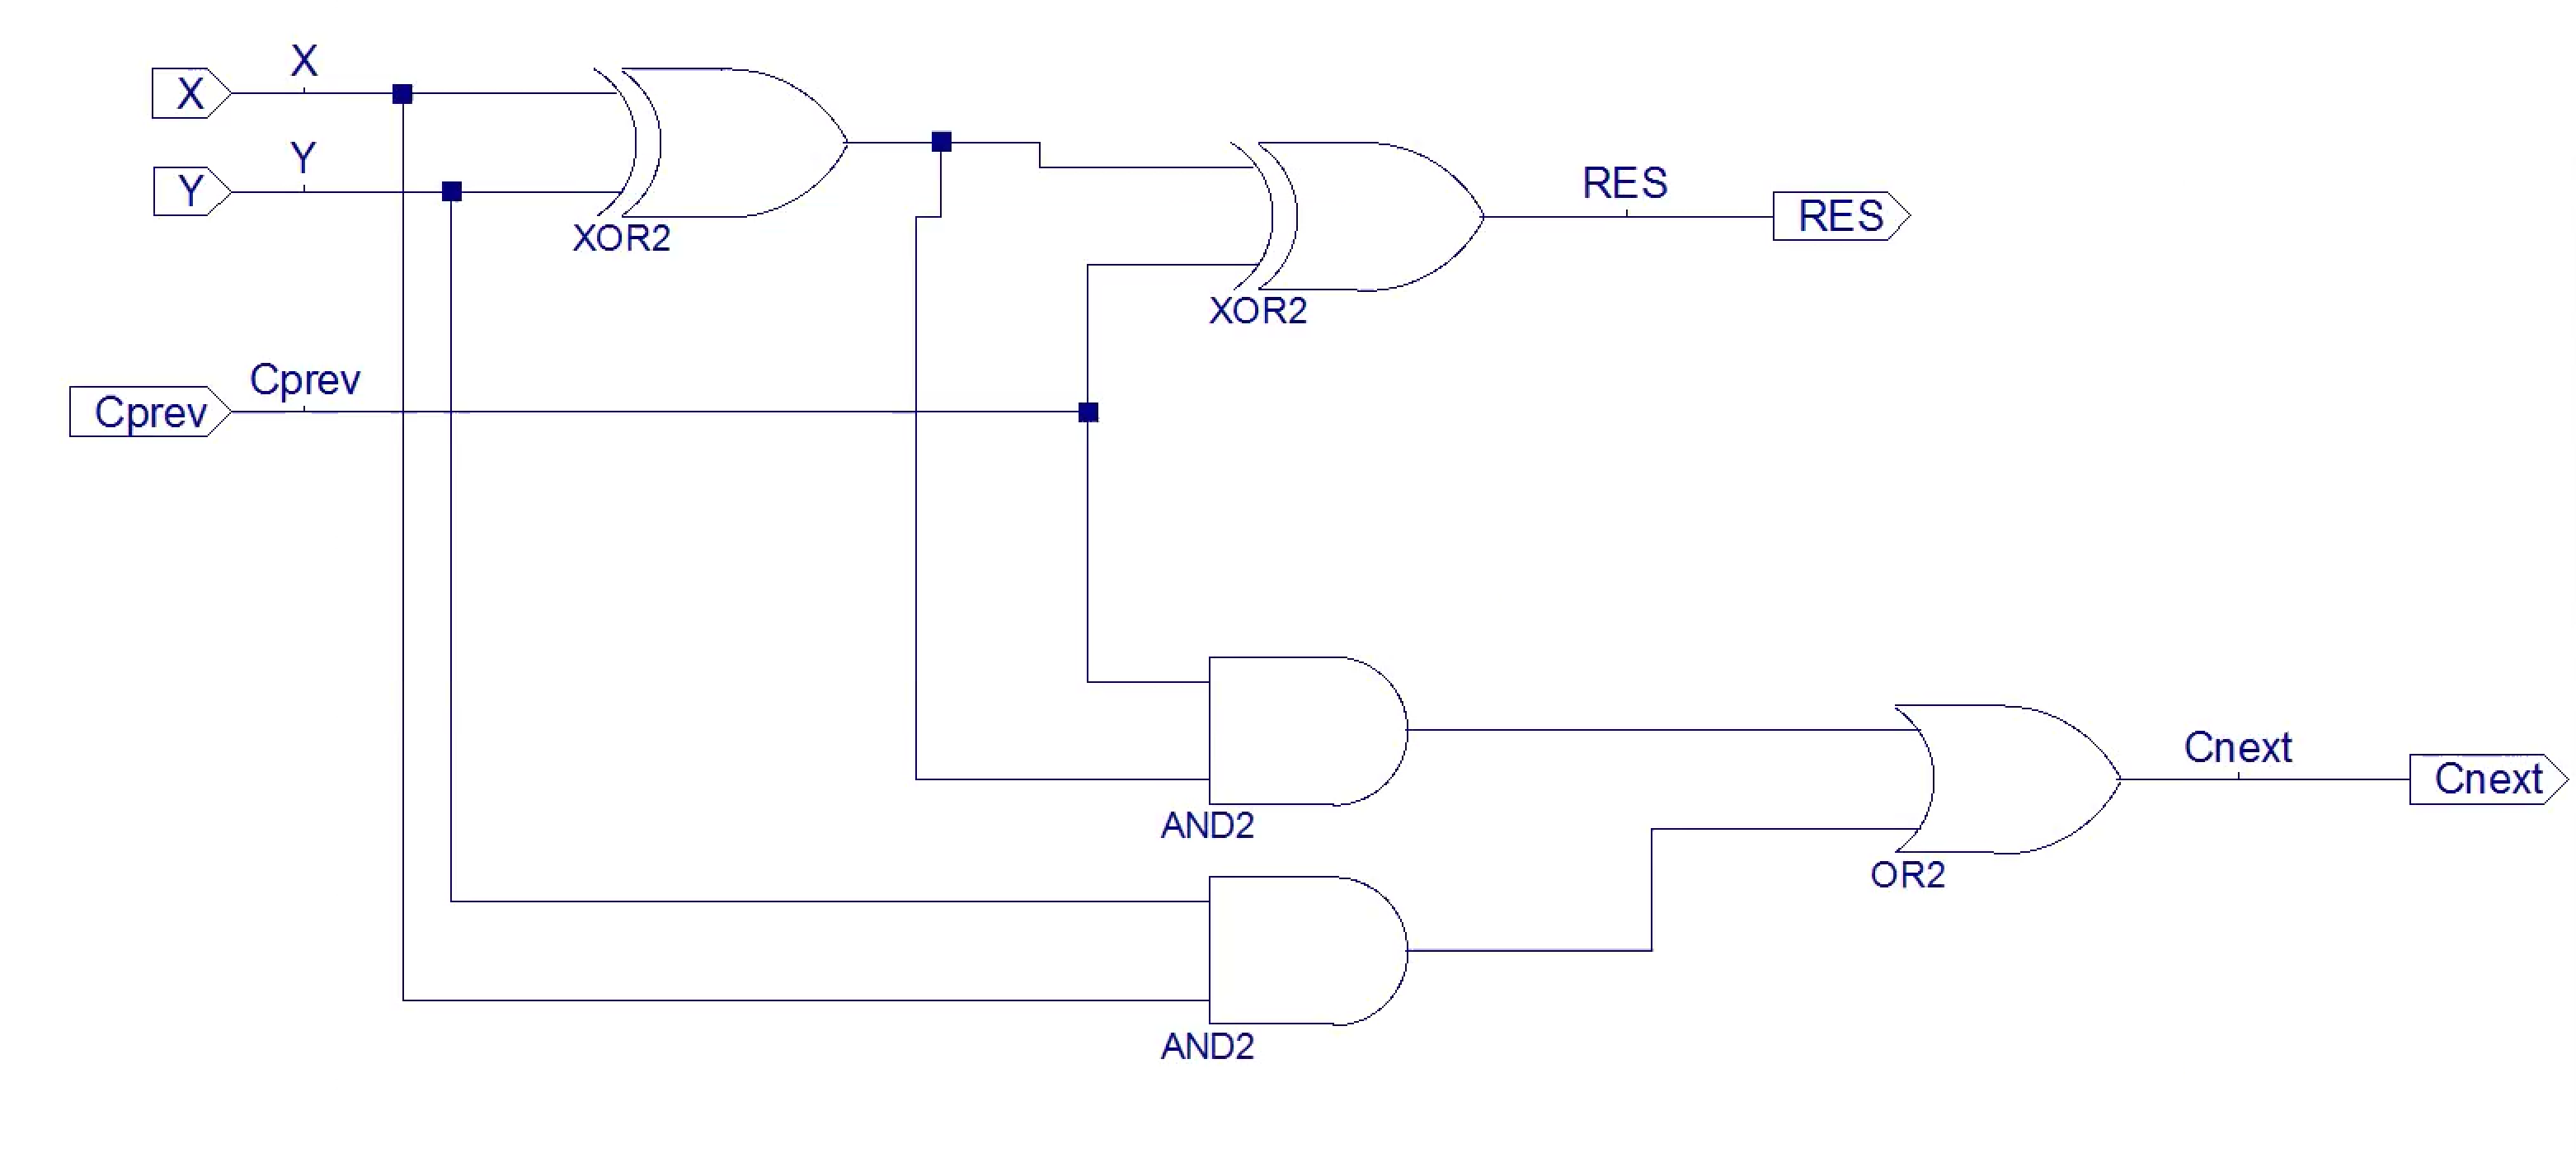
\includegraphics[scale=.3]{fa_sch.png}
		\end{center}
		
		\begin{Verbatim}[frame=single, fontsize=\small]
`timescale 1ns/1ps

module fa_tbw_tb_0;
    reg Cprev = 1'b0;
    reg X = 1'b0;
    reg Y = 1'b0;
    wire Cnext;
    wire RES;

fa_sch UUT(
.Cprev(Cprev),
.X(X),
.Y(Y),
.Cnext(Cnext),
.RES(RES));

initial begin
#100;

//CASE 1
X=0;
Y=0;
Cprev=0;
#100;

//CASE 2
X=0;
Y=0;
Cprev=1;
#100;

//CASE 3
X=0;
Y=1;
Cprev=0;
#100;

//CASE 4
X=0;
Y=1;
Cprev=1;
#100;

//CASE 5
X=1;
Y=0;
Cprev=0;
#100;

//CASE 6
X=1;
Y=0;
Cprev=1;
#100;

//CASE 7
X=1;
Y=1;
Cprev=0;
#100;

//CASE 8
X=1;
Y=1;
Cprev=1;
#100;

end
	
endmodule
		\end{Verbatim}
		
		We then can add onto this by adding the ability to subtract and making it 8-bit, thus creating an 8-bit adder/subtractor
		
		\begin{center}
			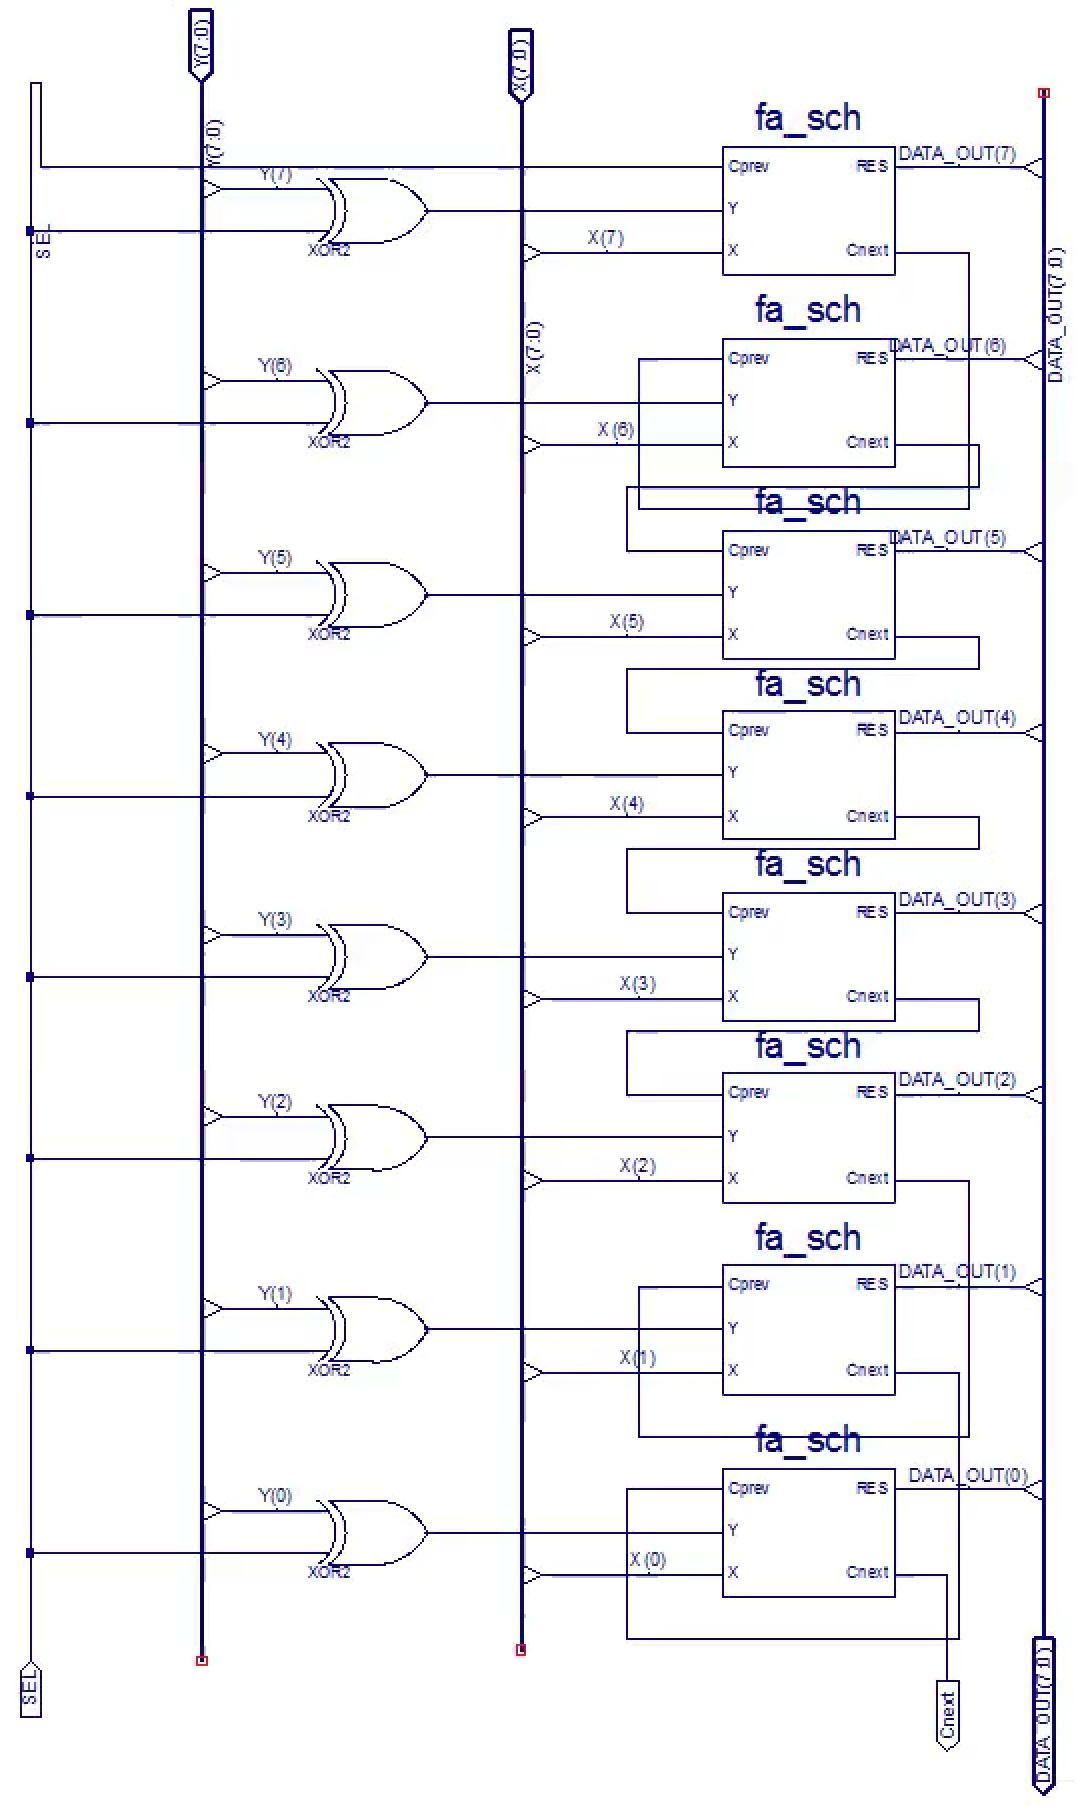
\includegraphics[scale=.5]{alu_sch.png}
		\end{center}
		
		\begin{Verbatim}[frame=single, fontsize= \small]
`timescale 1ns / 1ps
//alu_sch_alu_sch_sch_tb
module alu_tbw_tb();

// Inputs
   reg [7:0] X = 8'b00000000;
   reg [7:0] Y = 8'b00000000;
   reg SEL = 1'b0;

// Output
   wire [7:0] DATA_OUT;
   wire Cnext;

// Instantiate the UUT
   alu_sch UUT (
		.X(X), 
		.DATA_OUT(DATA_OUT), 
		.Cnext(Cnext), 
		.Y(Y), 
		.SEL(SEL)
   );
// Initialize Inputs
initial begin     
#100;   //Wait 100ns for initial inputs to settle.      
for (i=0; i<max_count; i=i+1)           
	begin             
		{X,Y,SEL} = i;  //Cycle through all input combinations.             
		#100;   //Wait 100ns between new inputs.         
	end 
end 
endmodule
			
		\end{Verbatim}

		
	\subsection{Part 1}
		Next, we built a logic extender so that we can output logic operations to the full adder.
		\begin{center}
			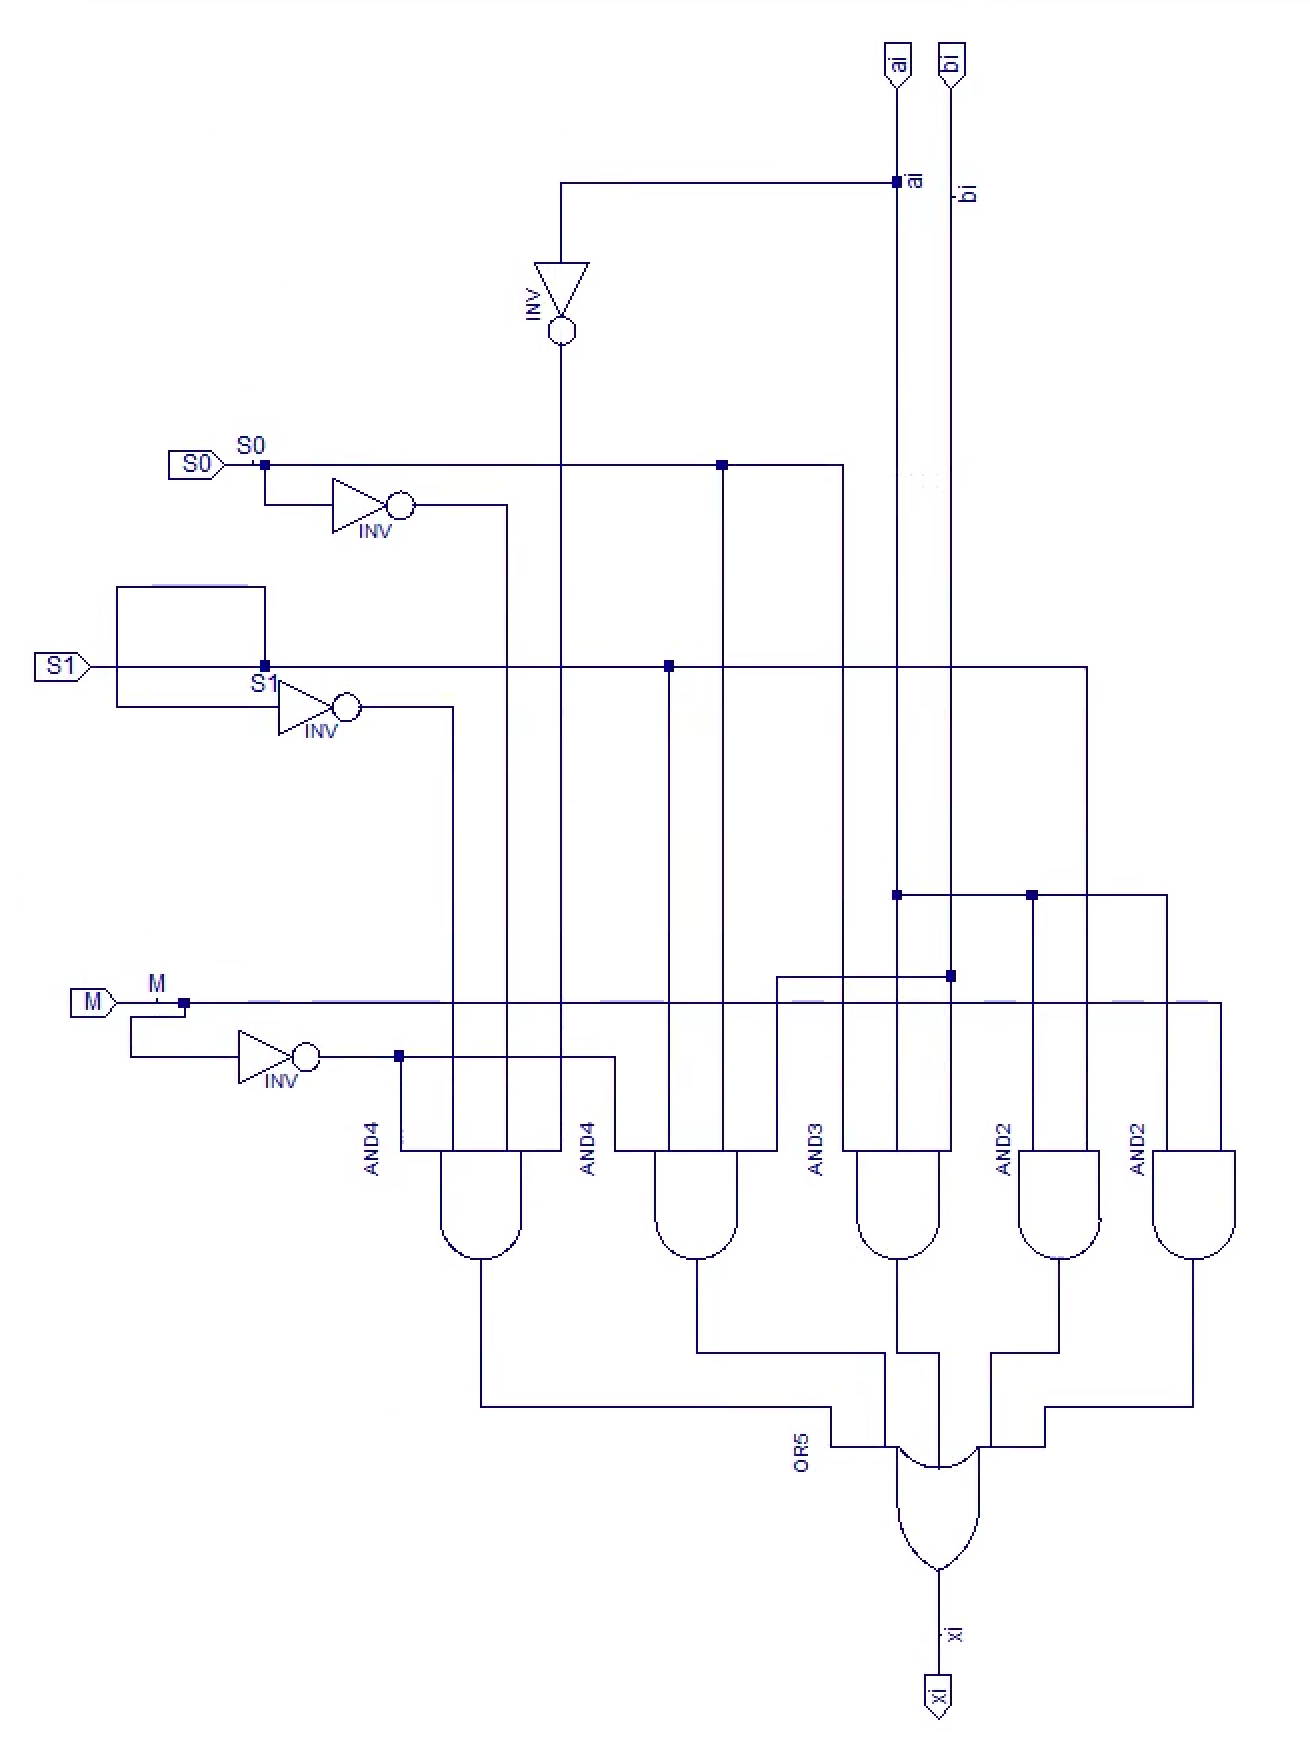
\includegraphics[scale=.5]{logic_ext_sch.png}
		\end{center}
	
		\begin{Verbatim}[frame=single, fontsize= \small]
`timescale 1ns / 1ps

module logic_ext_tbw_tb_0;

// Inputs
   reg ai;
   reg bi;
   reg S0;
   reg S1;
   reg M;

// Output
   wire xi;
	
	integer i = 0; 
	parameter num_inputs = 5; 
	parameter max_count = (1<<num_inputs);

// Instantiate the UUT
   logic_ext UUT (
		.xi(xi), 
		.ai(ai), 
		.bi(bi), 
		.S0(S0), 
		.S1(S1), 
		.M(M)
   );
// Initialize Inputs
       initial begin
#100;
 for (i=0; i<max_count; i=i+1)
	begin {M,S1,S0,ai,bi} = i; 
	#100; 
	end
end
endmodule			
		\end{Verbatim}

	
	\subsection{Part 2}
		Similar to the Logic Extender, we will build an Arithmetic extender, which forwards arithmetic operations to the full adder rather than logic ones.
		
		\begin{center}
			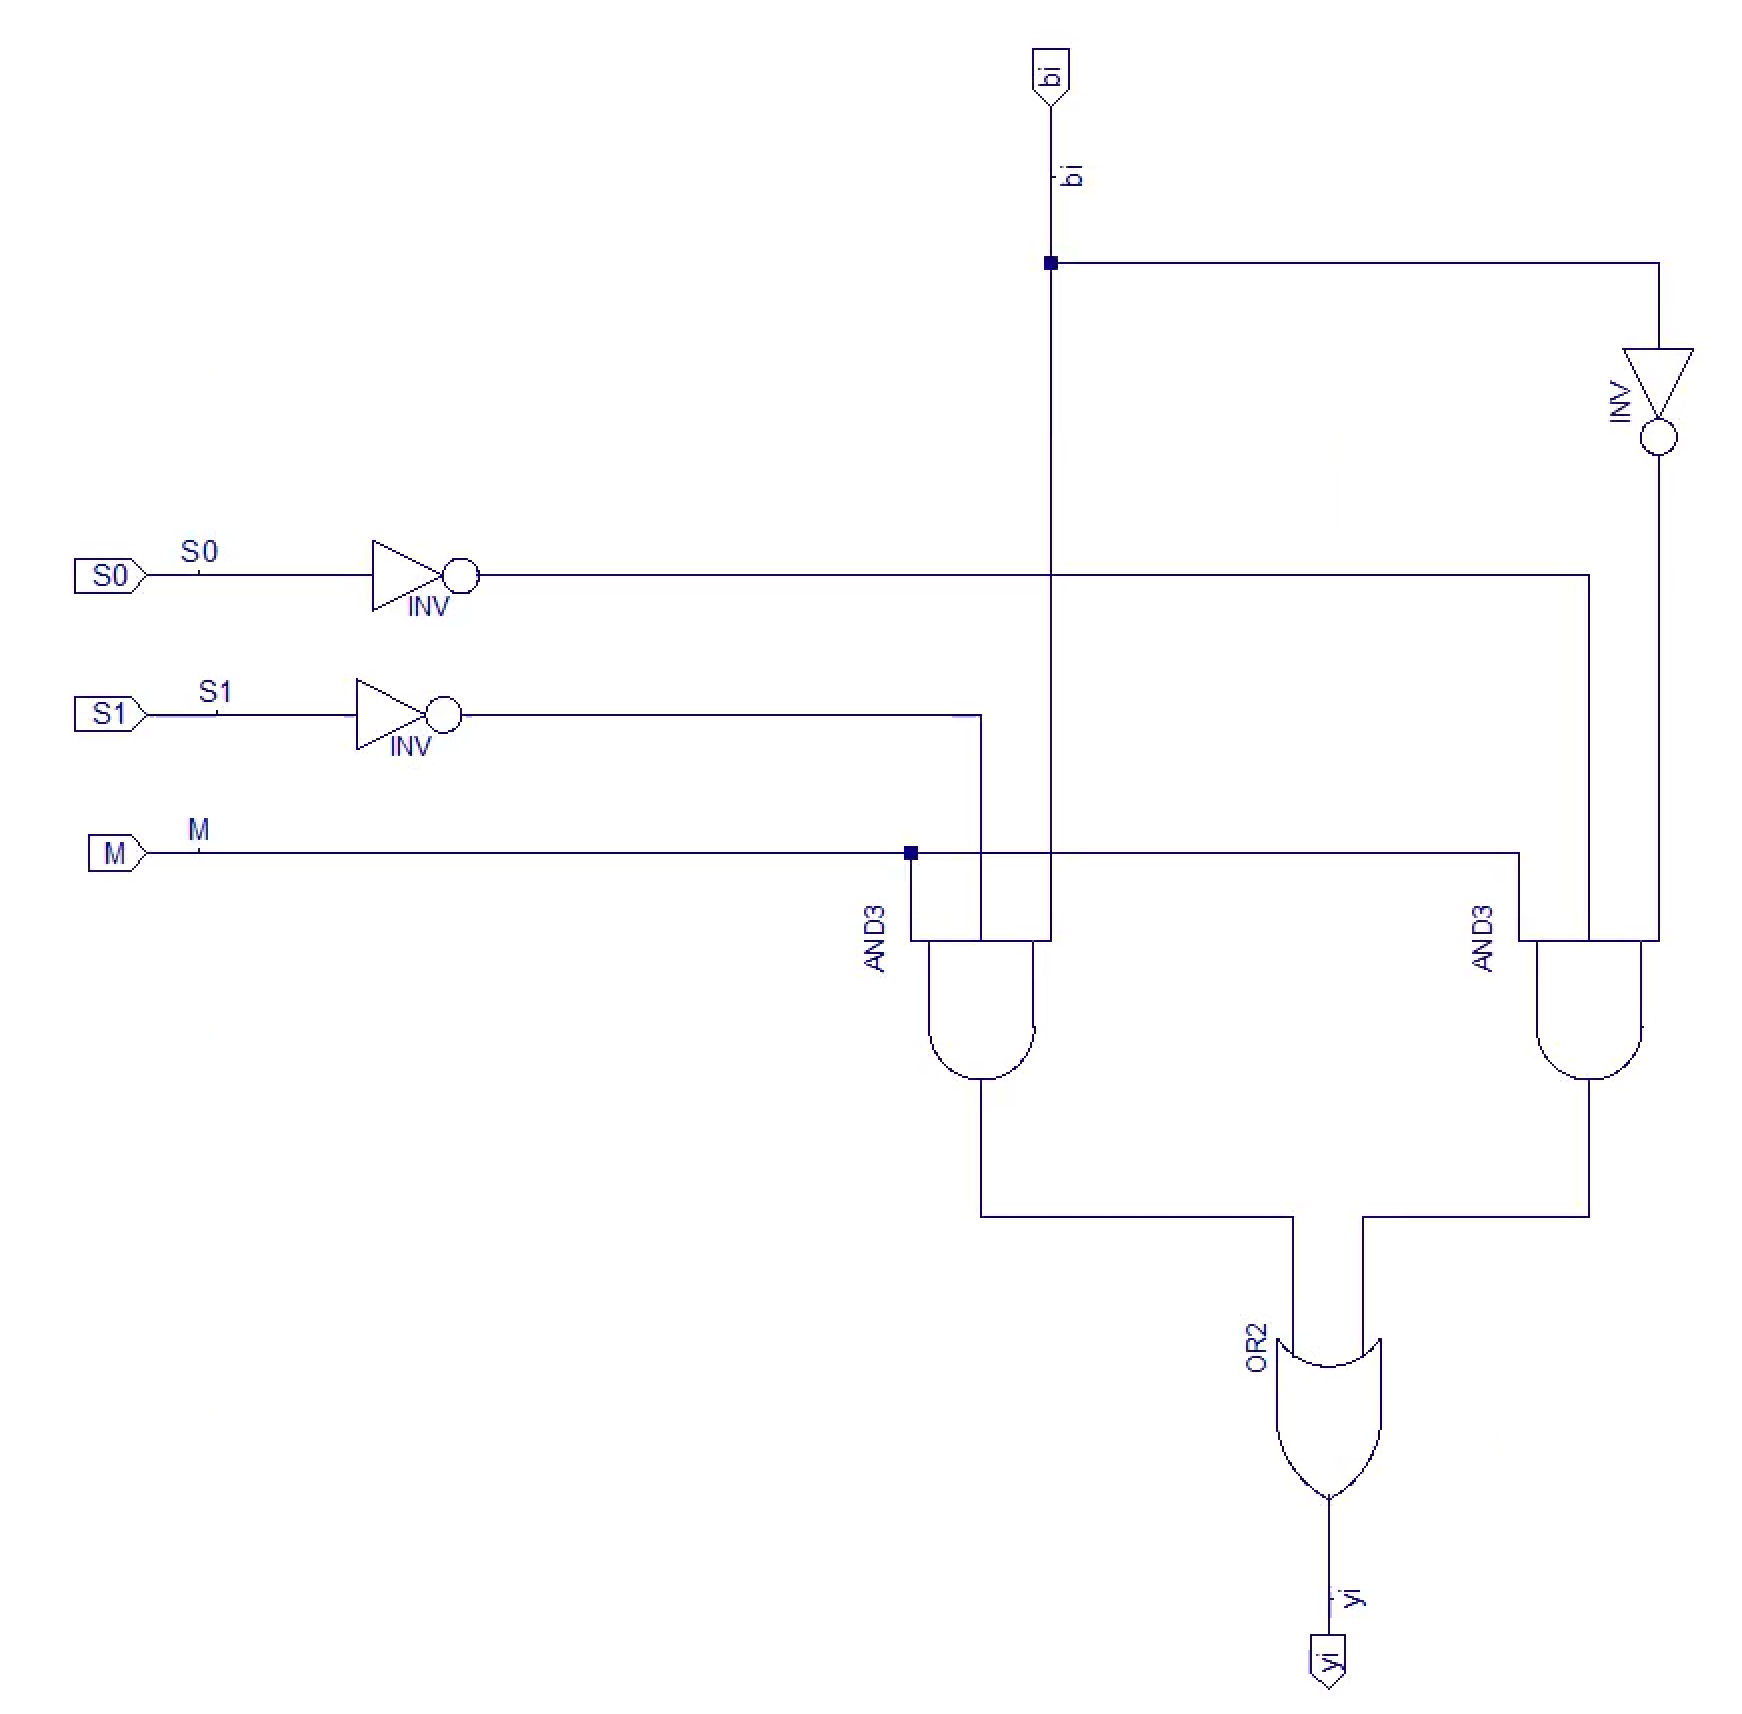
\includegraphics[scale=.5]{arith_ext_sch.png}
		\end{center}

		\begin{Verbatim}[frame=single, fontsize=\small]
`timescale 1ns/1ps 
module arith_ext_tbw_tb_0;     
reg bi = 1'b0;     
reg M = 1'b0;     
reg S0 = 1'b0;     
reg S1 = 1'b0;     
wire yi;     
integer i = 0;    
parameter num_inputs = 4;     
parameter max_count = (1<<num_inputs); 
 
arith_ext UUT (     
.bi(bi),     
.M(M),     
.S0(S0),     
.S1(S1),     
.yi(yi)); 
  
initial begin     
#100;   //Wait 100ns for initial inputs to settle.      
for (i=0; i<max_count; i=i+1)           
	begin             
		{M,S1,S0,bi} = i;  //Cycle through all 4 input combinations.             
		#100;   //Wait 100ns between new inputs.         
	end 
end 
 
endmodule 
			
		\end{Verbatim}

	\subsection{Part 3}
		Now we can combine the previous parts into a working 4-bit ALU. In essence, we stack the Logic Extender and the Arithmetic Extender onto the Full Adder
		\begin{center}
			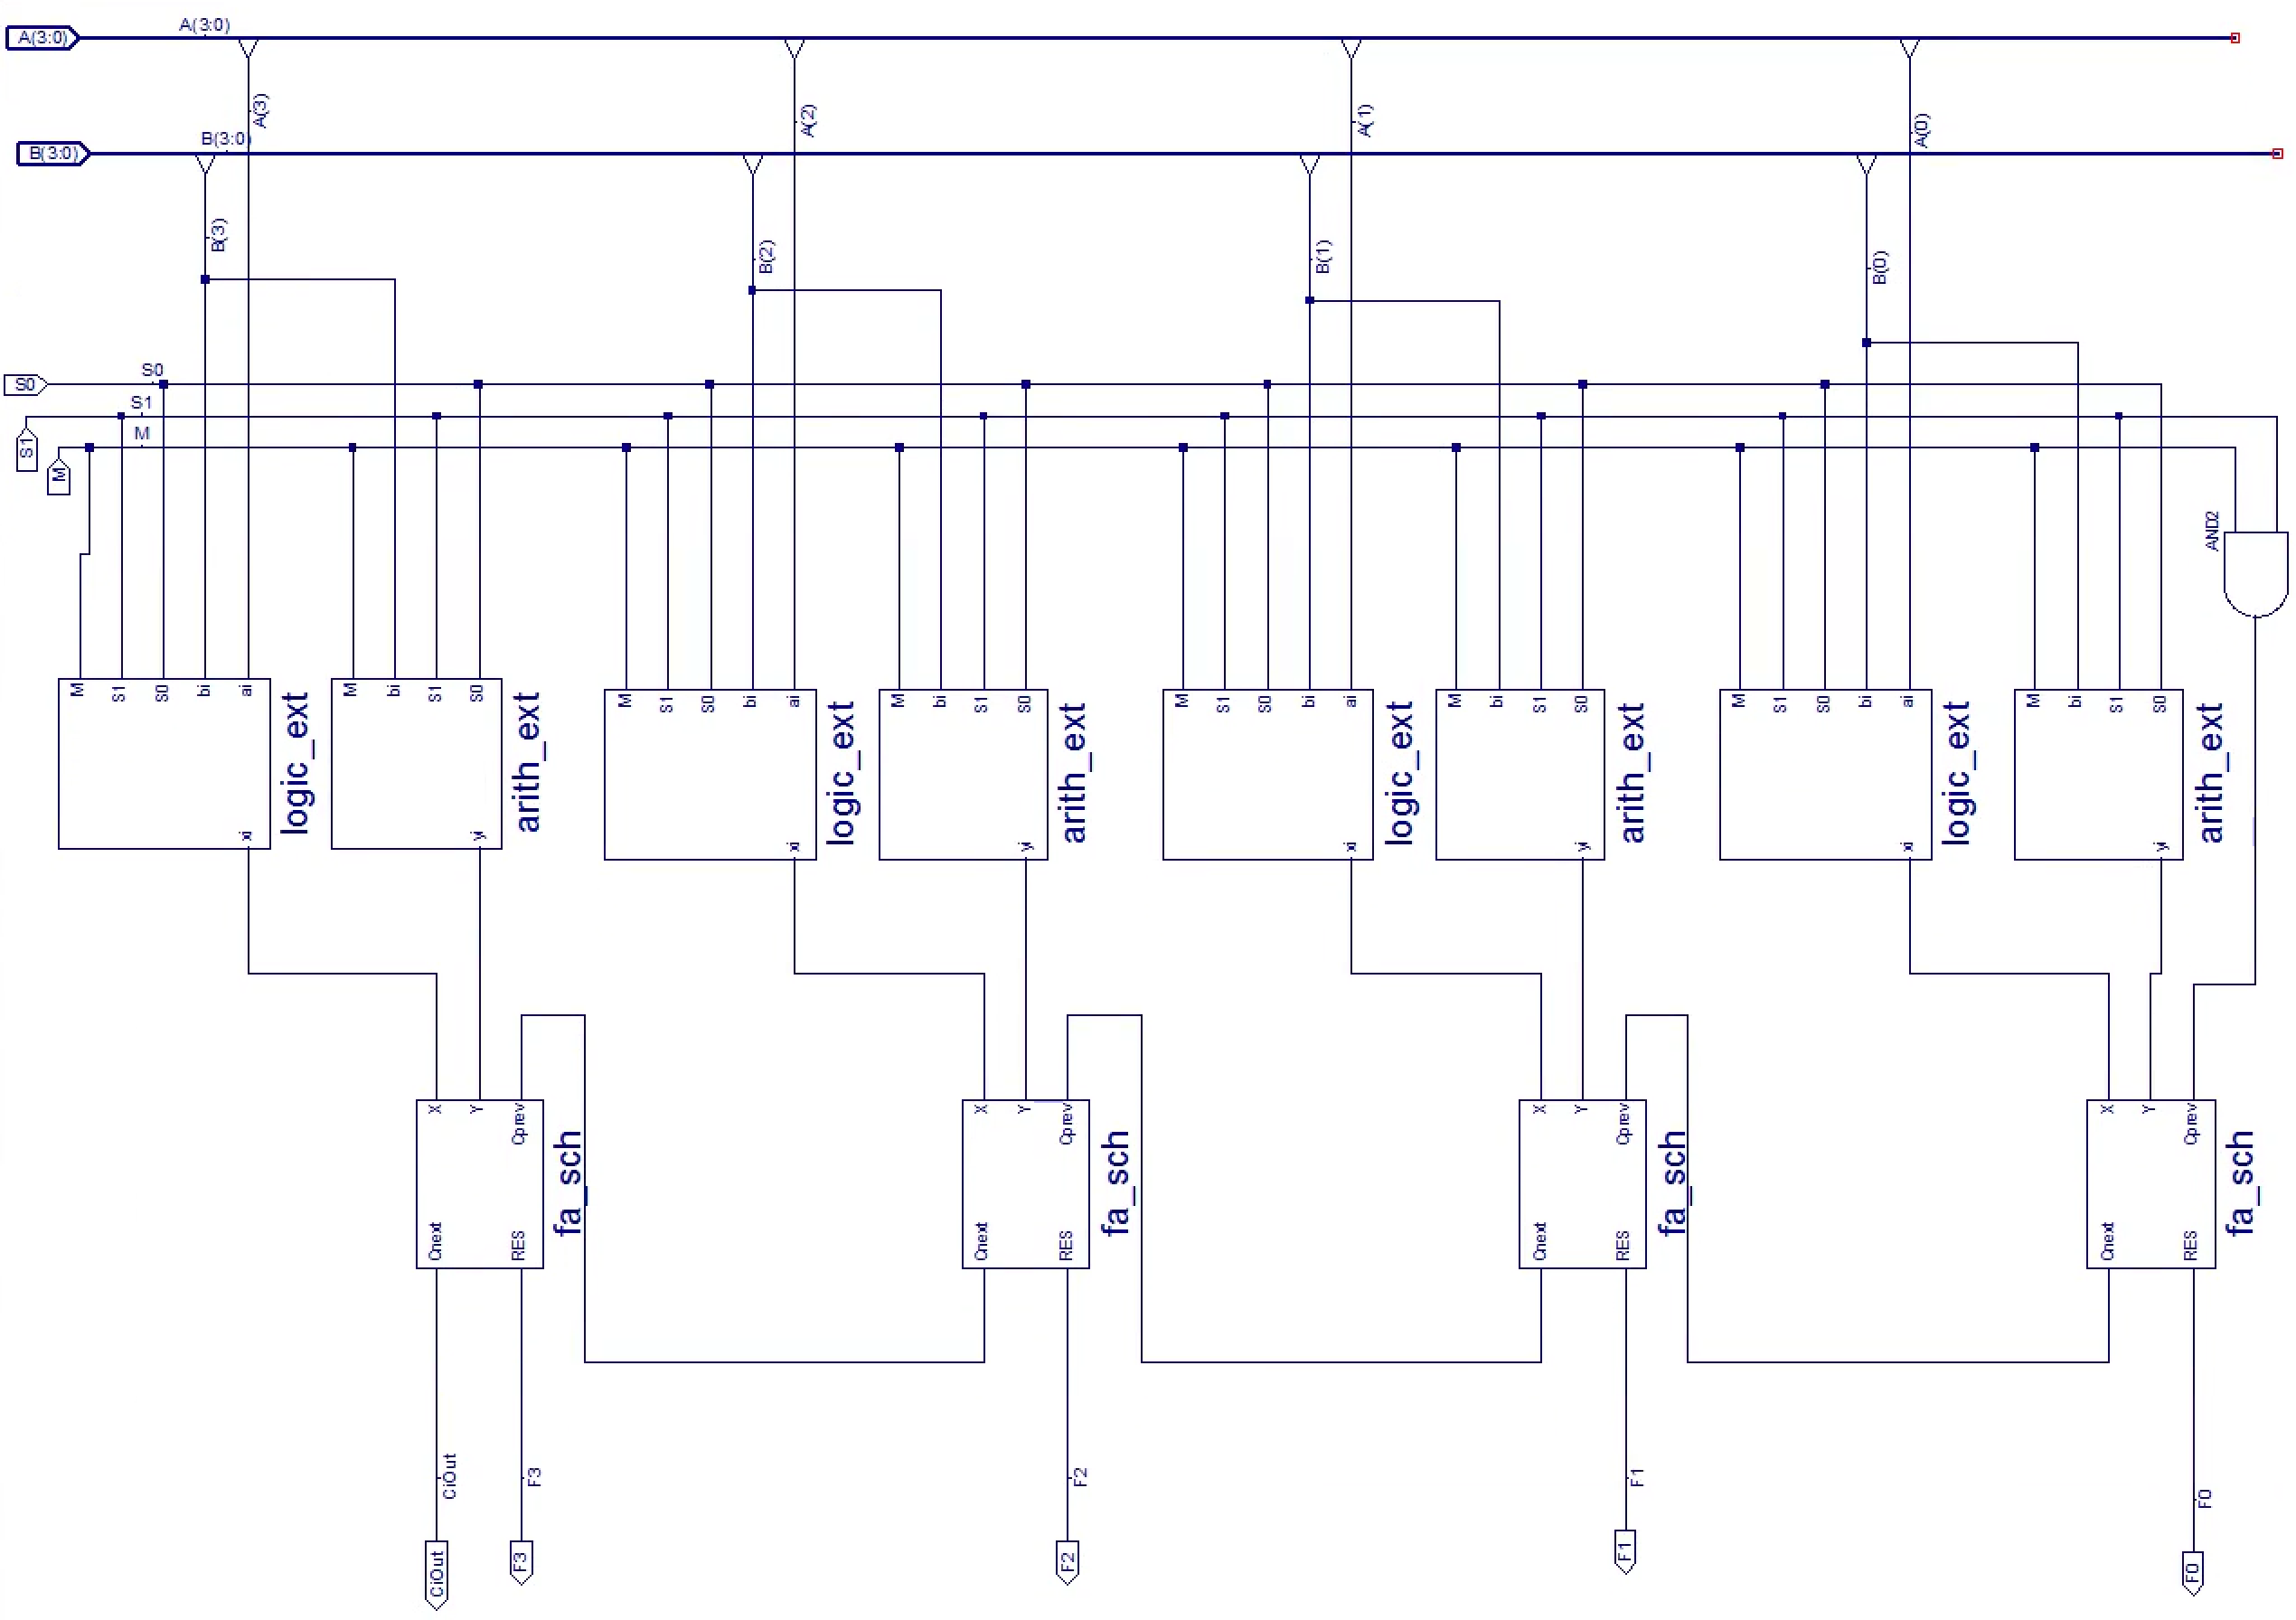
\includegraphics[scale=.3]{alu4bit_sch.png}
		\end{center}

		\begin{Verbatim}[frame=single, fontsize=\small]
`timescale 1ns / 1ps

module  alu4bit_tbw_tb_0;

// Inputs
   reg [3:0] A;
   reg [3:0] B;
   reg S0;
   reg S1;
   reg M;

// Output
   wire CiOut;
   wire F3;
   wire F2;
   wire F1;
   wire F0;

integer i =0;
parameter num_inputs =3;
parameter max_count = (1<<num_inputs);

// Instantiate the UUT
   alu4bit_sch UUT (
		.A(A), 
		.B(B), 
		.S0(S0), 
		.S1(S1), 
		.M(M), 
		.CiOut(CiOut), 
		.F3(F3), 
		.F2(F2), 
		.F1(F1), 
		.F0(F0)
   );
// Initialize Inputs

initial begin
#100;
for(i=0; i<max_count;i=i+1)
		begin
			{M,S1,S0}=i;
			A=4'b0101;
			B=4'b0100;
			#100;
		end
	#100;
	for(i=0; i<max_count;i=i+1)
		begin
			{M,S1,S0}=i;
			A=4'b1010;
			B=4'b0101;
			#100;
		end
	end
endmodule
			
		\end{Verbatim}

	
	\subsection{Part 4}
	
	\subsection{Part 5}
		Put together all of the parts with instruction of the given schematic. Tested everything per usual with a test bench.
	\subsection{Part 6}
		With the schematics in place and tests ran, a UCF file can be created to implement on the board.
		
		\begin{Verbatim}[frame=single, fontsize=\small]
NET "A(3)" LOC = "N3";
NET "A(2)" LOC = "E2";
NET "A(1)" LOC = "F3";
NET "A(0)" LOC = "G3";

NET "B(3)" LOC = "B4";
NET "B(2)" LOC = "K3";
NET "B(1)" LOC = "L3";
NET "B(0)" LOC = "P11";

NET "M"   LOC = "A7";
NET "S1"  LOC = "M4";
NET "S0"  LOC = "C11";

NET "CiOut" LOC = "G1";
NET "CLK"  LOC = "B8";

NET "F3" LOC = "P6";
NET "F2" LOC = "P7";
NET "F1" LOC = "M11";
NET "F0" LOC = "M5";

NET "SS(0)" LOC = "L14";
NET "SS(1)" LOC = "H12";
NET "SS(2)" LOC = "N14";
NET "SS(3)" LOC = "N11";
NET "SS(4)" LOC = "P12";
NET "SS(5)" LOC = "L13";
NET "SS(6)" LOC = "M12";

NET "EN_L"  LOC = "K14";
NET "EN_ML" LOC = "M13";
NET "EN_MR" LOC = "J12";
NET "EN_R"  LOC = "F12";			
		\end{Verbatim}

	
	\subsection{Part 7}
		Programmed the board, implemented our program on it, and ran through every logic and arithmetic operation in demonstration. Everything worked perfectly after some debugging.
			
\section{Experimental Results}\vspace{-.7cm} \line(1,0){470}

\begin{center}
	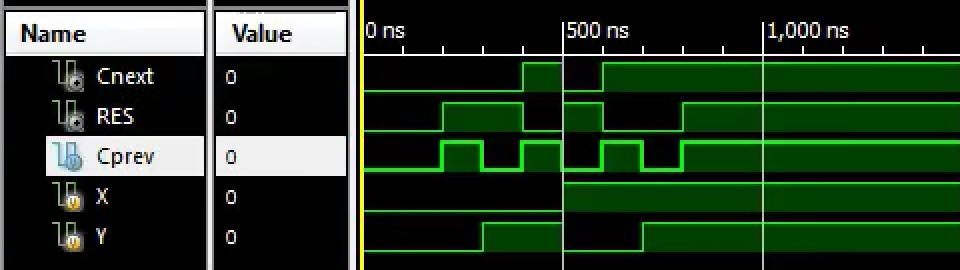
\includegraphics[scale=.7]{fa_tb_wave.png}
\end{center}

\begin{center}
	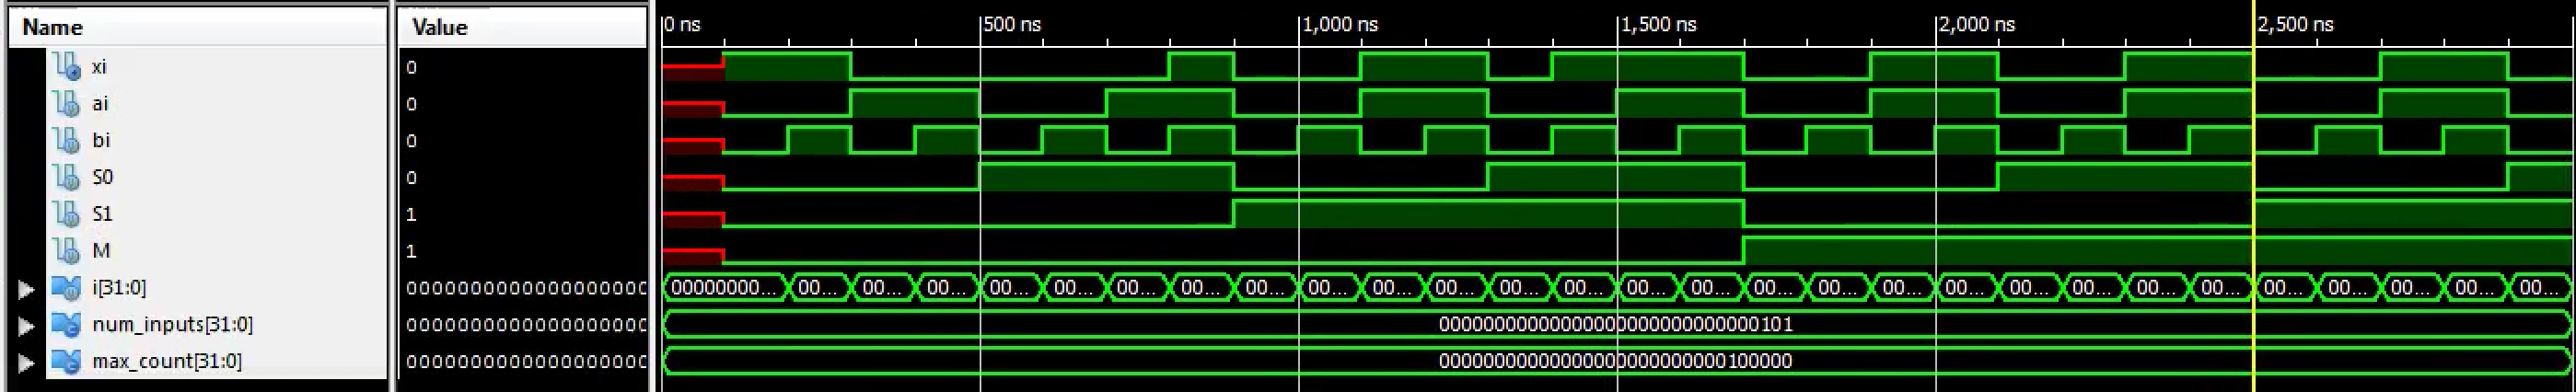
\includegraphics[scale=.33]{logic_ext_tb_wave}
\end{center}

\begin{center}
	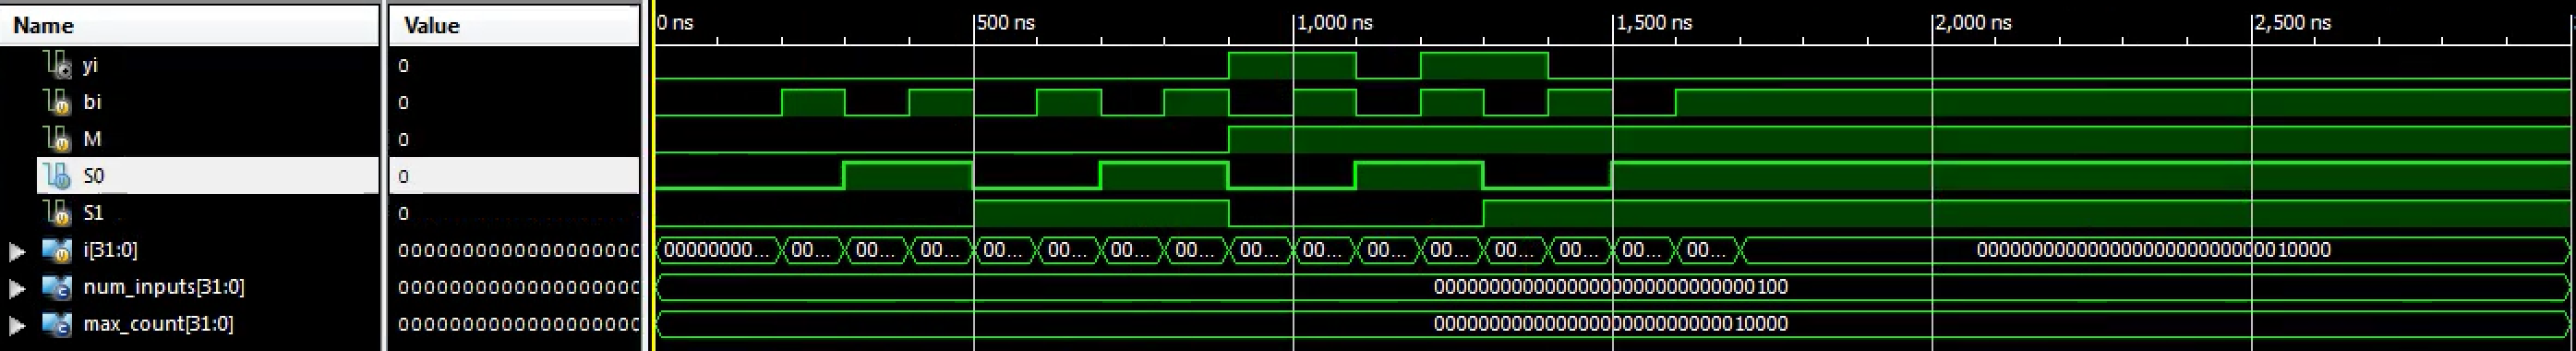
\includegraphics[scale=.33]{arith_ext_tb_wave.png}
\end{center}

\begin{center}
	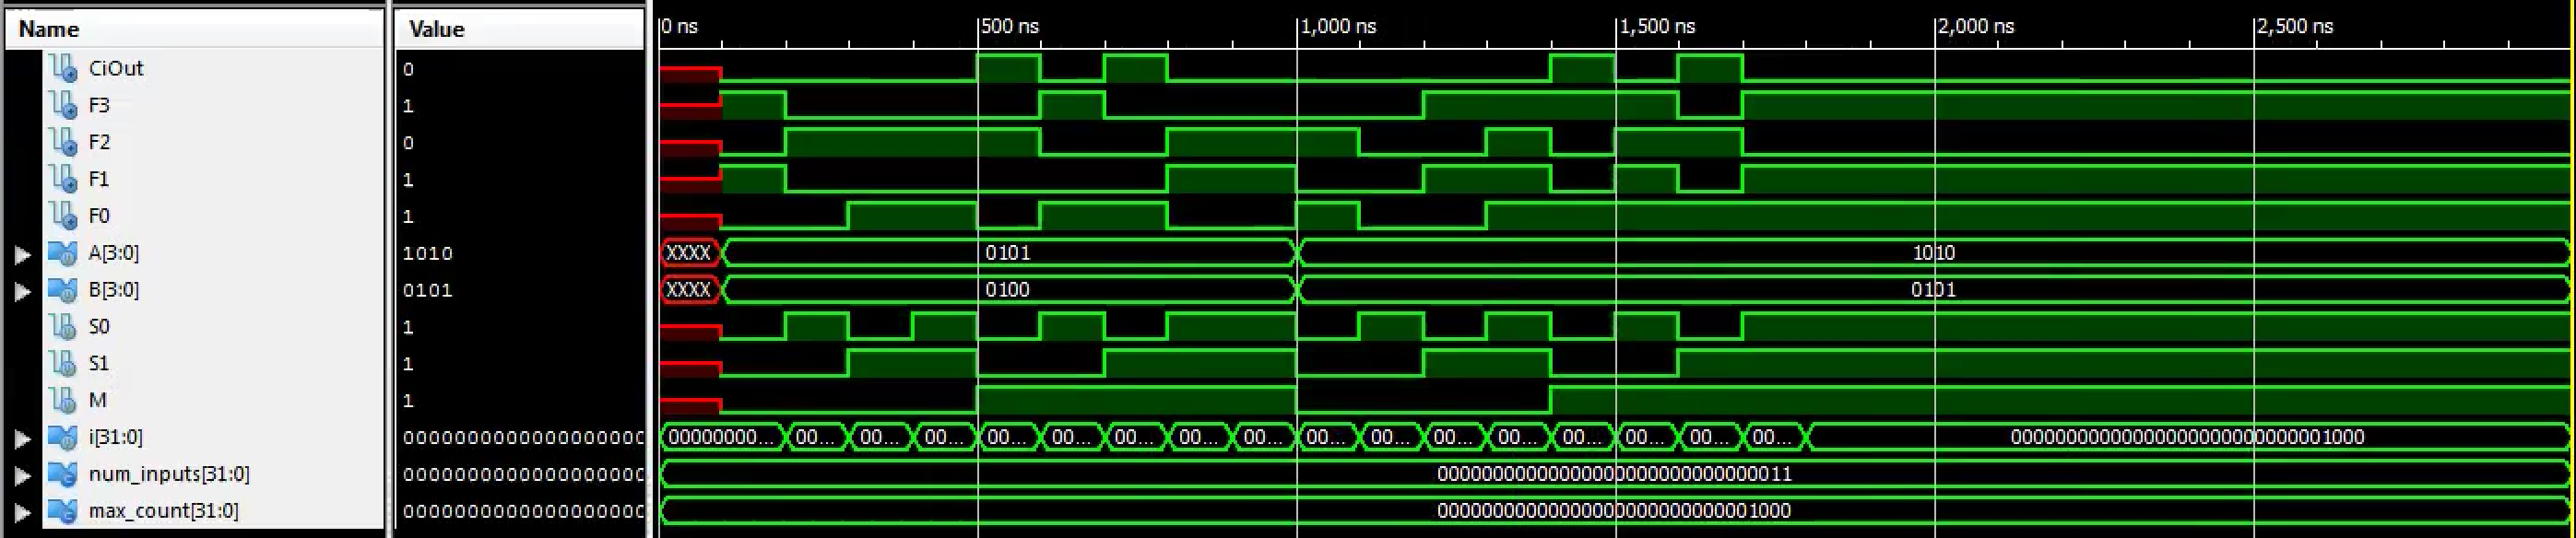
\includegraphics[scale=.33]{alu4bit_tb_wave.png}
\end{center}

			
\section{Significance} \vspace{-.7cm} \line(1,0){470}
	\paragraph{}
		

 \section{Comments/Suggestions}\vspace{-.7cm} \line(1,0){470}
 	\paragraph{}

		
\end{document}


